
\item A wooden block performs SHM on a frictionless surface with frequency, \( v_0 \). The block carries a charge \( +Q \) on its surface. If now a uniform electric field \( \vec{E} \) is switched-on as shown, then the SHM of the block will be
    \begin{center}
        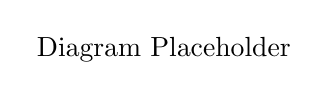
\begin{tikzpicture}
            % Since the actual diagram is not provided in text, you would need to recreate it or insert it as an image.
            \node at (0, 0) {Diagram Placeholder}; % Replace with diagram creation code
        \end{tikzpicture}
    \end{center}
    \begin{tasks}(2)
        \task of the same frequency and with shifted mean position.
        \task of the same frequency and with the same mean position.
        \task of changed frequency and with shifted mean position.
        \task of changed frequency and with the same mean position.
    \end{tasks}
